\section{Abstract}
The International Union for Conservation of Nature (IUCN) lists more than 70,000 species worldwide as endangered.
While a multitude of factors exert detrimental effects on the velocity of the extinction rate wildlife trade clocks in as the second biggest threat.
Many trades are considered illegal and categorize as poaching.
However, legal trades play a crucial role in the negative impact as well.
This visualization aims to raise awareness about the magnitude of global wildlife trade on the population of endangered species. It provides an interactive world map highlighting wildlife populations and trade activity between countries. Users are able to explore the visualization in temporal and geospatial space.

\section{Concept}
%\textbf{Introduce the story/concept with reasons why it's important to communicate about wildlife and endangered species trade}
\begin{quote}
"Our natural world is becoming increasingly vulnerable. We
know that effective conservation can yield outstanding
results, saving species from extinction while securing
the livelihoods of local communities. The international
community must urgently step up conservation efforts
if we want to secure this fascinating diversity of life
that sustains, inspires and amazes us every day." \\
- Inger Andersen, IUCN Director General \cite{Mauverney2012}
\end{quote}

% Currently, the number of endangered species on the IUCN Red List currently is more than 77,300\cite{Mauverney2012}. 

It is very hard to exactly determine how many species go extinct every year, because it is not clear exactly how many species there are to begin with. The lowest estimate of the amount of species on planet earth is 2 million. It is estimated that the current extinction rate is 1000 to 10000 times higher than the natural extinction rate. With this number, it is calculated between 0.01 and 0.1 percent of all species are going extinct each year. This means that even if this lowest estimate is true, between 200 and 2000 species go extinct every year. \footnote {WWF about biodiversity: \url{http://wwf.panda.org/about_our_earth/biodiversity/biodiversity/}, accessed: 23-02-2018} There are multiple reasons for this increase in biodiversity loss. Habitat destruction being the biggest. The second biggest threat to species' survival is wildlife trade. \footnote {WWF on biodiversity threats: \url{http://wwf.panda.org/about_our_earth/biodiversity/threatsto_biodiversity/}, accessed: 23-02-2018} \footnote {Influence of pet trade on many animal species: \url{https://theconversation.com/trading-in-extinction-how-the-pet-trade-is-killing-off-many-animal-species-71571}, accessed: 23-02-2018} \footnote {WWF on illegal trade: \url{http://wwf.panda.org/about_our_earth/species/problems/illegal_trade/}, accessed: 23-02-2018}

Many of the trades contributing to this wildlife threat are illegal. However, legal trades might actually play a role in this as well. Many of the zoos, pet sellers and aquariums used to rely on certified breeders for their animals. But it has been brought to light by the WWF that it might be possible that these animals were not bred in captivity, but snatched from their natural habitat. This would mean it is classified as legal trade, but the animals are actually illegally acquired \cite{trafficWWF} \cite{Nijman2015}. Another example where illegal trade is covered up by legal trade is the ivory business in Hong-Kong. It is claimed by traders that it is easy to launder the ivory, using the legal stockpile as front while selling the illegal, poached ivory. \cite{Lo2015}

%https://www.alternet.org/animal-rights/study-reveals-how-legal-trade-african-animals-pushing-several-species-extinction
%https://www.awf.org/campaigns/wildlife-trade-and-seizure-maps/


There is a growing worldwide concern with regard to the trade of endangered wildlife species. CITES\footnote {The Convention on International Trade in Endangered Species of Wild Fauna and Flora: \url{https://www.cites.org/eng/disc/what.php}, accessed: 23-02-2018} (the Convention on International Trade in Endangered Species of Wild Fauna and Flora) is the international agreement between 183 governments that aims to protect specimens of wild animals and plants from extinction through international trade.


\subsection{What we want to communicate}
To communicate awareness about the severity of trading endangered animal species, we propose an interactive visualization that shows the global endangered species population versus how much legal trade in these species has been recorded. By selecting a smaller subset of endangered animal species and specifying a time-frame, the visualization has the ability of telling the story of how legal trade of endangered animal species still contributes to a decline in population of that species in the wild.


\subsection{How do we want to communicate this?}
The visualization will be built around a full-screen world map on which countries are separated by their borders. This global view shows the trade between countries in the form of a connection map (Figure \ref{conmap}). By clicking specific connections, the map zooms in and shows more information regarding the trade, species, etcetera. A different map-mode is the \textit{choropleth} map (Figure \ref{choropleth}), which illustrates the global endangered species population for a subset of species per country. By pressing a button, map-modes can be switched easily. A timeline at the bottom of the map makes it possible to see changes in endangered animals population and legal international trade. 
Apart from viewing the different relationships between endangered species, trades and countries, the individual countries can also be clicked. When an individual country is selected, the user can see which species are imported in to that country and which species are exported from that country. Furthermore, the user can see an aggregated view of the purpose of the imported species for that specific country.
\begin{figure} [h]
\begin{subfigure}{.5\columnwidth}
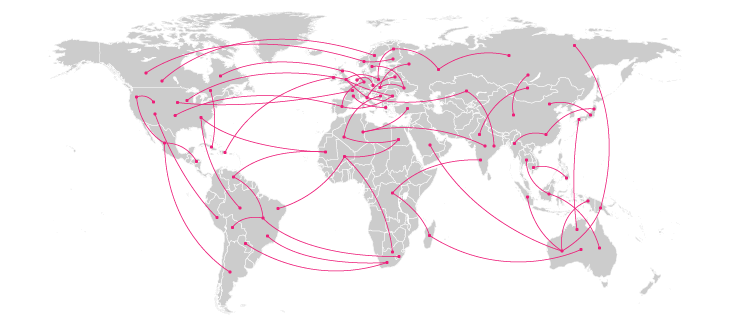
\includegraphics[width=6cm]{images/connection_map.png}
\caption{Example of a Connection Map}
\label{conmap}
\end{subfigure}
\begin{subfigure}{.5\columnwidth}
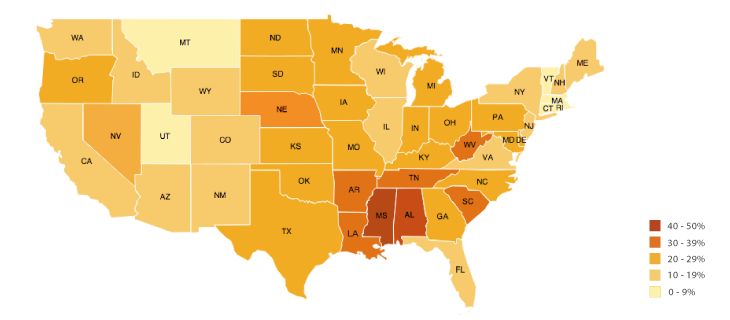
\includegraphics[width=6cm]{images/choropleth.png}
\caption{Example of a Choropleth Map}
\label{choropleth}
\end{subfigure}
\caption{}
\label{}
\end{figure}


% - Focus on animal species
% - Global but distinction between countries
% - Alive/Death Animals -> As a filter option
% - Awareness of trade of endangered species by showing the population of a species (in the wild) versus the trade going on.
% - Purpose, distinction between purpose
% - Time (temporal), more than one year
% - What does endangered mean?
% - How many species do live in the wild versus how much trade is there.



\iffalse %<this is the beginning of the section that I am commenting out of the preview

\subsection{Idea 1 }
\textbf{Exporting specimen that are taken from the Wild between 2007 and 2017.}
(\textit{by querying \href{https://trade.cites.org/en/cites_trade/}{CITIES Trade Database} twice, once from 2007-2011 and once from 2012-2017 and then merging them in excel, easy peasy. or if that is too big, we can do it per year and merge them. I VOLUNTEER if others find this too much work =D }) \\

Story we can communicate: \\
Since this is a database on trade of \textbf{endangered} species. We can communicate a story surrounding the endangered species in this database. We can surely find information from the past 10 years that will tell us more about when certain species became endangered and we can then relate that to numbers going up or down in terms of export. We can also show which countries "contribute" to this export and maybe pick the biggest purposes and show them.\\

Using multi-view we can show two things: \\
Left side showing a \href{https://datavizcatalogue.com/methods/stacked_area_graph.html}{stacked area map} of the species that are exported (or only the top 5 - 10 or something) in which you can see how this has changed over the past 10 years. Or another graph that shows something like this. Right side showing a worldmap, maybe a \href{https://datavizcatalogue.com/methods/flow_map.html}{flow map}, to show the flow around the world. User is able to switch between years?

\begin{figure} [h] \label{visid1}
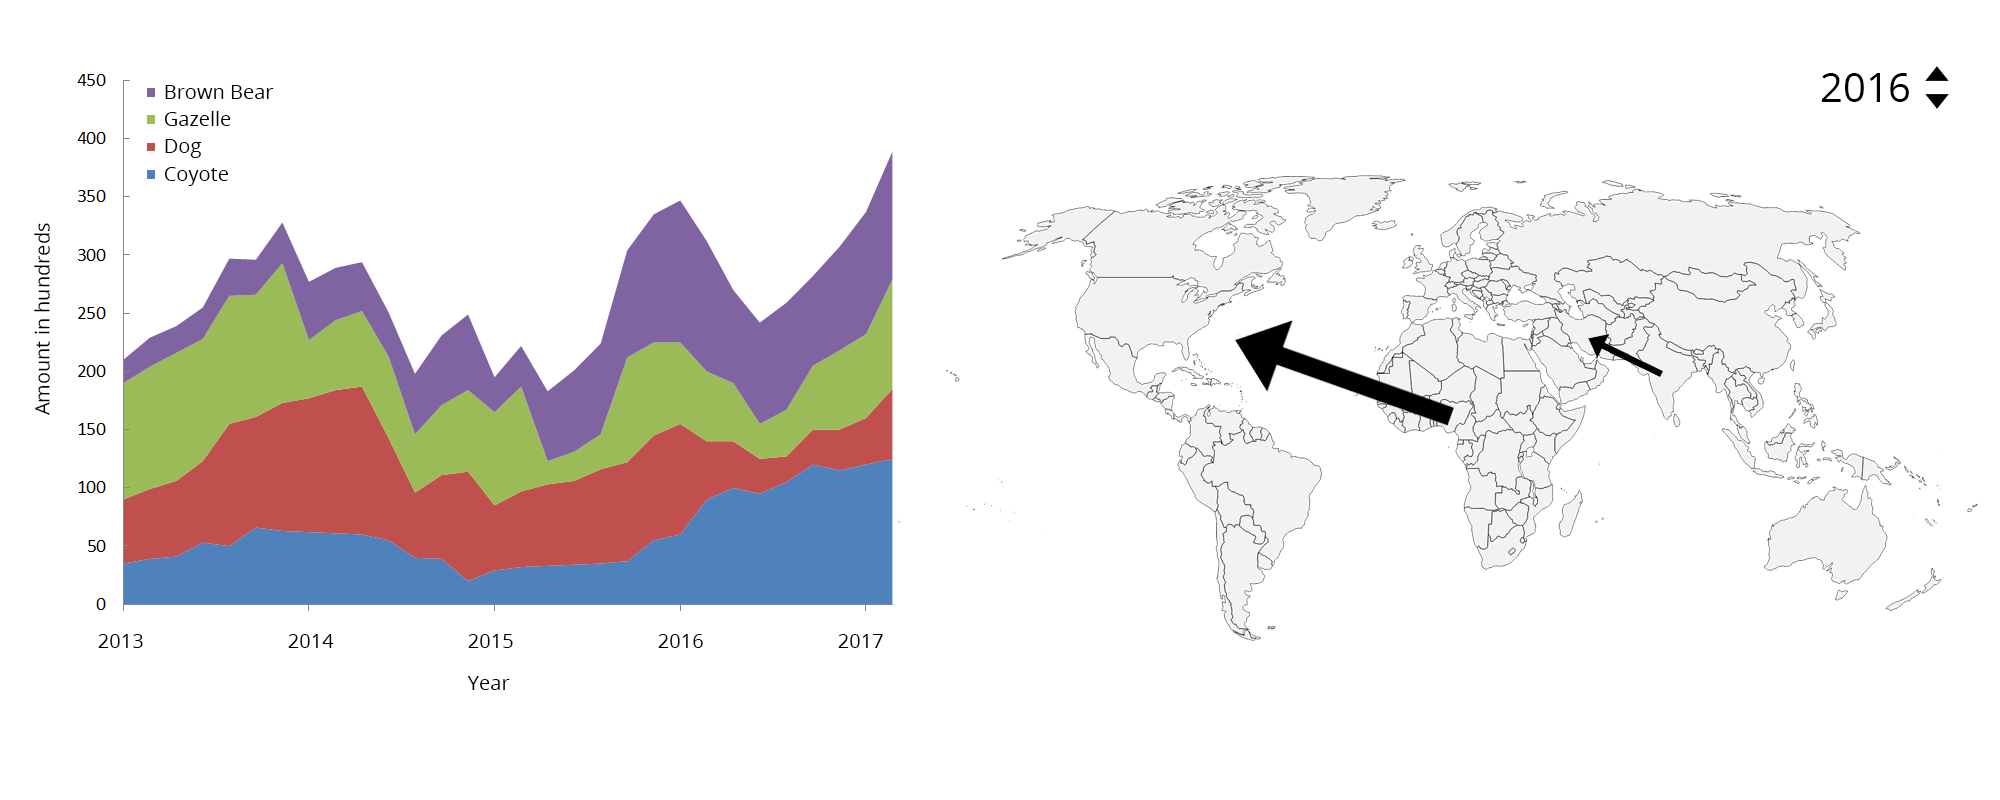
\includegraphics[width=12cm]{images/idea1-maaike.png}
\caption{}
\end{figure}

\subsection{Idea 2 }
\textbf{Import/export with medical purpose from 2007-2017} = One big map with different interaction possibilities\\

This visualization shows who exports and who imports the wildlife with a \href{https://datavizcatalogue.com/methods/connection_map.html}{Connection Map} for example. Zooming out combines the connections and makes the lines thicker (each species maybe has another color?) and zooming in gives more detail. Users can click a line and see more information about what is being imported/exported, by whom and the quantity.  \href{https://i.pinimg.com/736x/1b/b8/27/1bb82777d0aca7ce9abd08441e06781e.jpg}{this} or \href{http://metrocosm.com/animated-immigration-map/}{this} or \href{https://www.mapd.com/demos/tweetmap/}{this} or \href{https://ecoregions2017.appspot.com/}{this} can be used for inspiration maybe.


\subsection{Visualization idea 3}
A world map showing which country exported and imported the most (maybe with a button?). A timeline at the bottom with tiptools marking when a species went extinct or acquired a new endangerment status. When a country is selected a new graphs shows up on the right or left containing information on which species it imported and exported and the quantity of it.

\begin{figure} [h] \label{visid2}
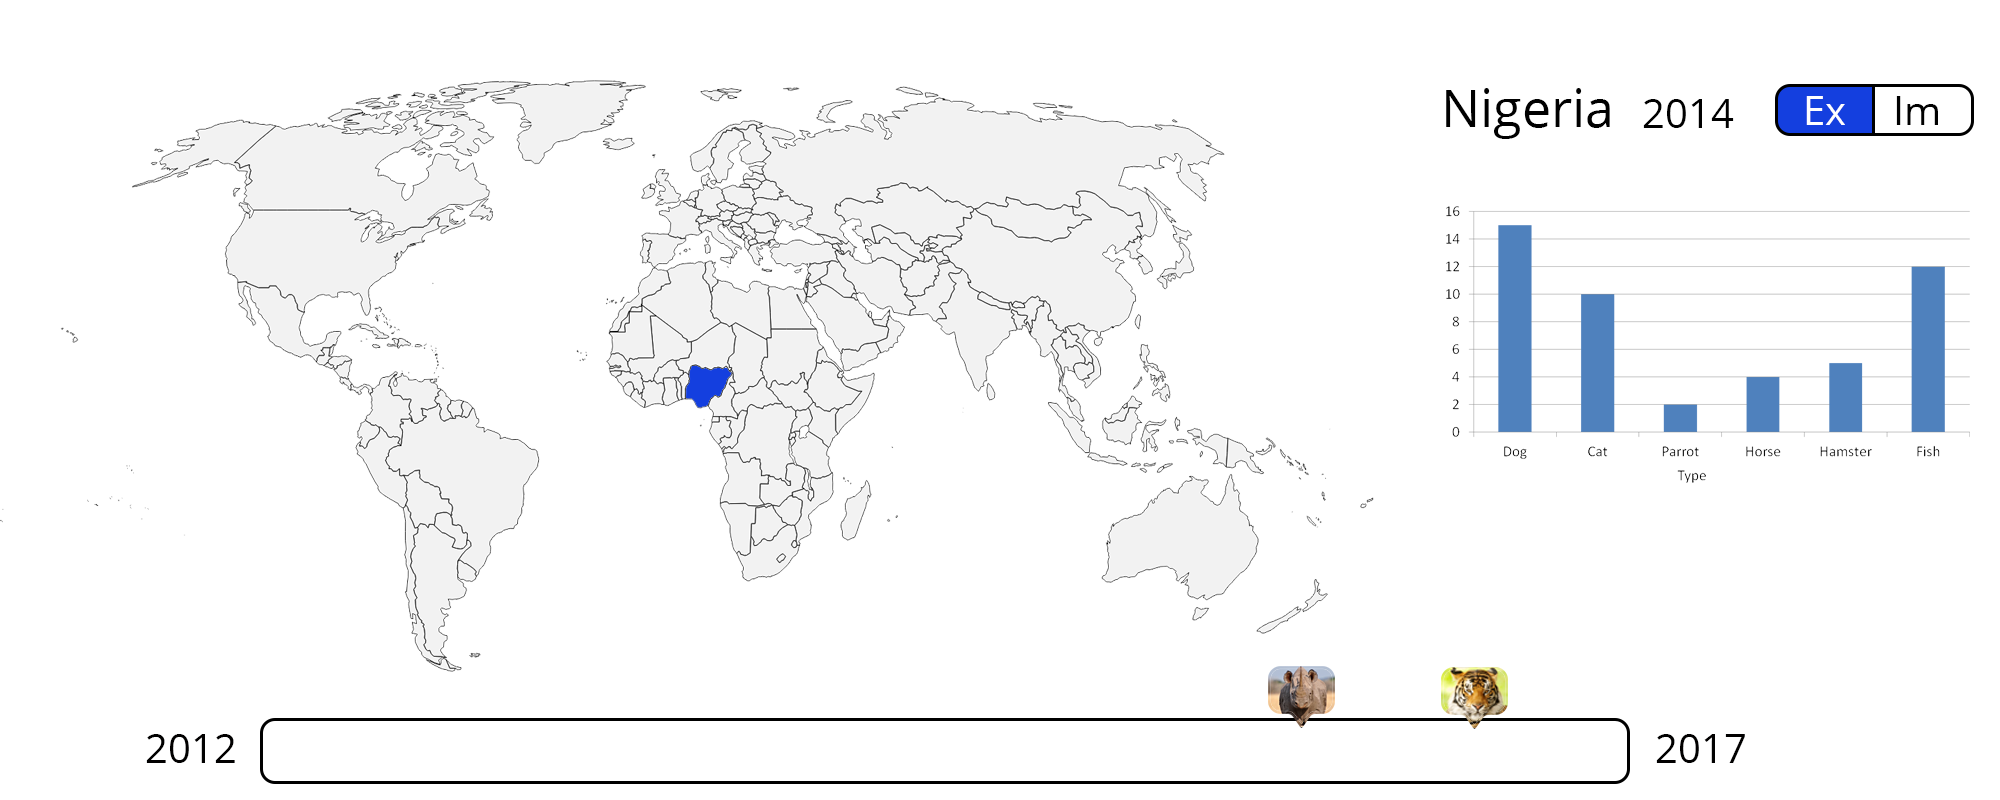
\includegraphics[width=12cm]{images/idea-infovis.png}
\caption{visualization idea 3}
\end{figure}

\fi %<this is the end of the section that I am commenting out of the preview






\iffalse %<this is the beginning of the section that I am commenting out of the preview
\textcolor{blue}{literal text from articles to help guide: } \\
"Creating a visualization requires a number of nuanced judgments. One must determine which questions to ask, identify the appropriate data, and select effective \textit{visual encodings} to map data values to graphical features such as position, size, shape, and color.
\begin{itemize}
\item \textbf{Time-Series Data} = Sets of values changing over time;
\begin{itemize}
\item \textbf{Stacked Area Map} \href{https://datavizcatalogue.com/methods/images/top_images/stacked_area_graph.png}{stacked area map}
\end{itemize}
\item \textbf{Statistical Distributions}  = to reveal how a set of numbers is distributed and thus help van analyst better understand the statistical properties of the data;
\item \textbf{Maps} = Many maps are based upon a \textit{cartographic projection}: a mathematical function that maps the 3D geometry of the earth to a 2D image. Other maps knowingly distort or abstract geographic features to tell a richer story or highlight specific data
\begin{itemize}
\item \textbf{Flow Maps} can depict the movement of a quantity in space and (implicitly) in time. Flow lines typically encode a large amount of multivariate information: path points, direction, line thickness, and color can all be used to present dimensions of information to the viewer.
\item \textbf{Choropleth Maps} Data is often collected and aggregated by geographical areas such as states. A standard approach to communicating this data is to use a color encoding of the geographic area, resulting in a \textit{choropleth map.}
\item \textbf{Graduated Symbol Maps} are an alternative to the choropleth map. The graduated symbol map places symbols over an underlying map. This approach avoids confounding geographic area with data values and allows for more dimensions to be visualized (for example, symbol size, shape, and color).
\item \textbf{Cartograms} A \textit{cartogram} distorts the shape of geographic regions so that the area directly encodes a data variable. A common example is to redraw every country in the world sizing it proportionally to population or gross domestic product.
\item \textbf{Heatmaps on maps}
\end{itemize}
\end{itemize}
\cite{Heer2010}. \\


\textbf{Multiview}; Some ways in which data sets can differ include \cite{Baldonado2000}:
\begin{itemize}
\item The dataset is a subset of another (e.g. the result of some filtering operation)
\item The dataset contains aggregates of the individual values of a second data set (e.g.  visualizations at different zoomlevels; one view might show average costs for each type of restaurant in an area, while a second view shows the location of each individual restaurant)
\item The data set contains entirely different information (e.g. one view shows the logical structure of an integrated circuit and another a detailed graphical layout representing the actual geometry of the circuit to be fabricated)
\end{itemize}
\fi %<this is the end of the section that I am commenting out of the preview


\section{Dataset}
The dataset on wildlife trade originates from the Convention on International Trade in Endangered Species of Wild Fauna and Flora (CITES). CITES is based on an international agreement between governments which aims to assure that international trade in specimens of wild animals and plants does not threaten their survival. CITES is financed from contributions from the parties of the convention based on the United Nations scale of assessment. \footnote {What is CITES?: \url{http://wwf.panda.org/about_our_earth/biodiversity/biodiversity/}, accessed: 27-02-2018}. Table 1 shows the dataset as described by CITES \footnote{CITES Wildlife Trade Database, Column Metadata: \url{https://www.kaggle.com/cites/cites-wildlife-trade-database/data}, accessed at 26-02-2018}.

\begin{table}[!ht]
\begin{tabular}{ l l p{8cm} }
\hline
\emph{Name} & \emph{Type} & \emph{Description} \\
\hline
Year & Integer & Year the export or import occurred \\ \hline
Appendix & String & Varying from I to III. I is most protected, III the least. \\ \hline 
Taxon & String & The species' taxonomic taxon \\ \hline 
Class & String & The species' taxonomic class \\ \hline 
Order & String & The species' taxonomic order \\ \hline 
Family & String & The species' taxonomic family \\ \hline 
Genus & String & The species' taxonomic genus or scientific name \\ \hline 
Importer & String & Abbrevation of the country in ISO-3166-1 importing the species \\ \hline 
Exporter & String & Abbrevation of the country in ISO-3166-1 exporting the species \\ \hline
Origin & String & Abbrevation of the country in ISO-3166-1 which the species originated \\ \hline
Import reported quantity & Integer & Quantity of the imported species' as reported to CITES. Blank if an export record. \\ \hline
Export reported quantity & Integer & Quantity of exported species' as reported to CITES. Blank is an import record. \\ \hline
Unit & String & Quantity type varying from 'g' for grams to 'lbs' for pounds. Default is unit quantity. \\ \hline
Purpose & String & The purpose with which the species was exported or imported. \\ \hline
Source & String & Describes how species was brought onto market. \\ \hline
\end{tabular}
\caption{Fields in the Wildlife dataset as described by CITES} \label{tbl:dataset-fields}
\end{table}

\section{Description of the data gathering process}

% \subsection{Information Retrieval}
% Which criteria was used to find a potential dataset? (?)

\subsection{Integration of different sources} \label{sec:source-integration}
To see which potential effect legal animal trade could have on the extinction rate of animals, connections are made with the IUCN Red List API \footnote{IUCN Red List API \url{http://apiv3.iucnredlist.org/api/v3/docs}} that focuses on endangered species. Extraction from this API has only been done for species that exist in the trade database. Because the data only shows trades that happened in the year 2016, no conclusions can be drawn on the influence this has on endangered species.



\subsection{Data Cleaning}
The following description is derived from the work of Rahm and Do \cite{Rahm2000DataApproaches}.
In its essence data cleaning aims to improve the overall quality of data.
This goal is achieved by removing errors, noise, duplicates, inconsistencies and misspellings from datasets.
Especially when multiple data sources are being integrated into a single set the need for data cleaning becomes apparent.
Different sources often feature varying representations of the same data.

As this visualization pulls in data from heterogeneous sources (Section \ref{sec:source-integration}) common data cleaning techniques are applied for consolidation.
There are four areas of concern: (1) Linking the scientific Latin name, (2) filtering non-animal entries, (3) enriching abbreviations with labels and (4) establishing a common relational schema.
The following sections elaborate on these areas in detail.

\subsubsection{Name Linking}
The \textit{Taxon} field of the CITES Wildlife dataset contains the scientific name of an animal in Latin.
While a direct connection to the IUCN API can be established using the Latin taxonomic name it is not suitable for data analysis (without a background in Biology) nor for usage in the final visualization.
Therefore, taxonomic names should be mapped to their English common counterpart.
Querying the IUCN API allows the retrieval of common names in one or more languages.

\begin{lstlisting}[caption={Retrieving common names of the red panda from the IUCN API}, label={lst:iucn-common-names}, language=json]
GET /species/common_names/ailurus%20fulgens
{
  "name": "Ailurus fulgens",
  "result": [
    {
      "taxonname": "Red Panda",
      "primary": true,
      "language": "eng"
    },
    ...
  ]
}
\end{lstlisting}

Collecting a unique set of taxonomic names provides the basis to iteratively query the IUCN API for common names. Listing \ref{lst:iucn-common-names} shows an example query for the red panda using a simple HTTP GET request.

\subsubsection{Non-animal Filter}
This visualization project intentionally focuses on animal wildlife only.
However, the CITES Wildlife database contains both animals and vegetation.
Each non-animal entry should therefore be filtered from the dataset.
There is no binary column indicating to which group an entry belongs.
Instead, the \textit{Term} field describes which type is being imported or exported.
Reducing the \textit{Term} column to its unique values yields 83 distinct types.
These types can manually be flagged when they signify non-animal entries e.g. seeds, dried plants, roots, bark, logs, fruit or leaves.

\subsubsection{Abbreviation Enrichment}
The CITES Wildlife database features five columns containing abbreviations: (1) \textit{Importer}, (2) \textit{Exporter}, (3) \textit{Origin}, (4) \textit{Purpose} and (5) \textit{Source}.
Cutting down the length of repetitive values helps to reduce file size and retains readability in editors.
In order to display these values in a visualization full labels should be used.
This provides an accurate description which does not rely on additional background knowledge.

\textit{Importer}, \textit{Exporter} and \textit{Origin} all contain two-letter country codes in the ISO 3166 alpha-2\footnote{\url{https://www.iso.org/iso-3166-country-codes.html}, accessed: 28-02-2018} format.
\textit{Purpose} and \textit{Source} are specific one-letter codes which can be resolved using the CITES trade guidelines documentation\footnote{\url{https://trade.cites.org/cites_trade_guidelines/en-CITES_Trade_Database_Guide.pdf}, accessed: 28-02-2018}.


\subsubsection{Relational Schema} 
\textcolor{white}{filler}

\begin{figure} [h] 
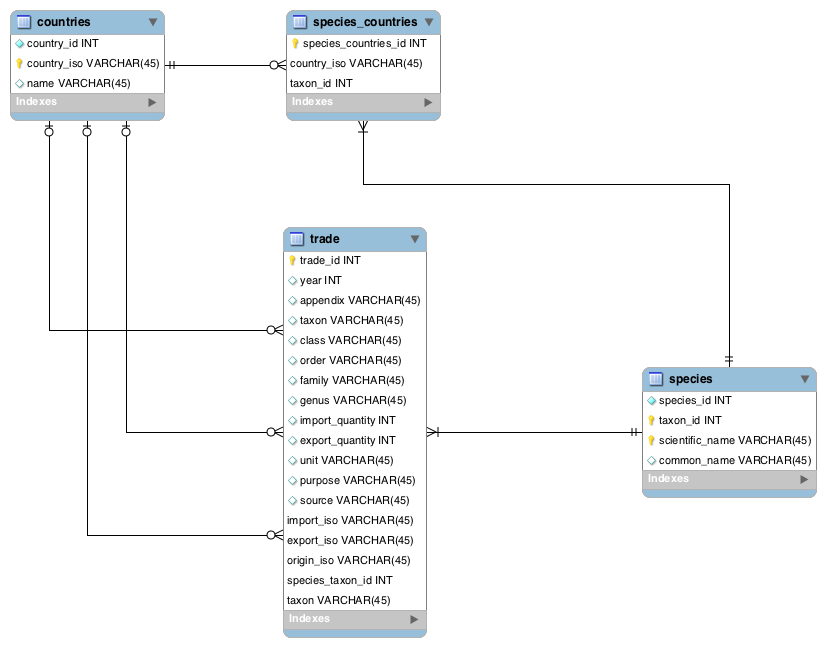
\includegraphics[width=12cm]{images/relation_schema.png}
\caption{Relational Schema}
\label{Relation Schema}
\end{figure}

